


\tikzset{every picture/.style={line width=0.75pt}} %set default line width to 0.75pt        

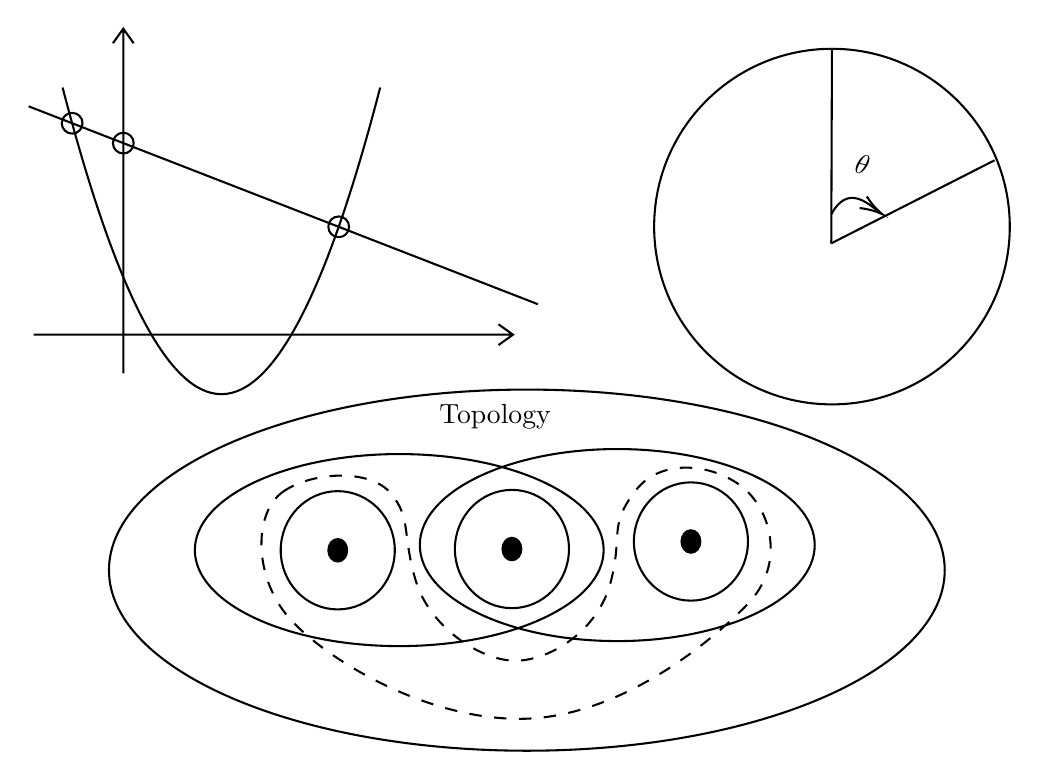
\begin{tikzpicture}[x=0.75pt,y=0.75pt,yscale=-1,xscale=1]
    %uncomment if require: \path (0,365); %set diagram left start at 0, and has height of 365

    %Shape: Axis 2D [id:dp3330650107827038] 
    \draw  (95.33,153.74) -- (326.33,153.74)(138.57,6.33) -- (138.57,172.41) (319.33,148.74) -- (326.33,153.74) -- (319.33,158.74) (133.57,13.33) -- (138.57,6.33) -- (143.57,13.33)  ;
    %Shape: Parabola [id:dp6747224874888704] 
    \draw   (109.33,34.67) .. controls (160.33,231.65) and (211.33,231.65) .. (262.33,34.67) ;
    %Straight Lines [id:da4045208158970277] 
    \draw    (93,43.74) -- (338.33,139.07) ;
    %Shape: Circle [id:dp9495260244967654] 
    \draw   (394.33,101.67) .. controls (394.33,54.35) and (432.69,16) .. (480,16) .. controls (527.31,16) and (565.67,54.35) .. (565.67,101.67) .. controls (565.67,148.98) and (527.31,187.33) .. (480,187.33) .. controls (432.69,187.33) and (394.33,148.98) .. (394.33,101.67) -- cycle ;
    %Straight Lines [id:da6440917457226727] 
    \draw    (480,16) -- (479.67,109.74) ;
    %Straight Lines [id:da2506243181764847] 
    \draw    (558.33,69.74) -- (479.67,109.74) ;
    %Curve Lines [id:da36631824919286937] 
    \draw    (479.67,95.74) .. controls (487.55,81.18) and (497.1,90.36) .. (502.77,94.64) ;
    \draw [shift={(504.33,95.74)}, rotate = 212.01] [color={rgb, 255:red, 0; green, 0; blue, 0 }  ][line width=0.75]    (10.93,-3.29) .. controls (6.95,-1.4) and (3.31,-0.3) .. (0,0) .. controls (3.31,0.3) and (6.95,1.4) .. (10.93,3.29)   ;
    %Shape: Ellipse [id:dp9329672718104849] 
    \draw   (131.67,267.19) .. controls (131.67,219.14) and (221.81,180.19) .. (333,180.19) .. controls (444.19,180.19) and (534.33,219.14) .. (534.33,267.19) .. controls (534.33,315.24) and (444.19,354.19) .. (333,354.19) .. controls (221.81,354.19) and (131.67,315.24) .. (131.67,267.19) -- cycle ;
    %Shape: Ellipse [id:dp9998724111128214] 
    \draw   (173.04,257.52) .. controls (173.04,231.97) and (217.13,211.26) .. (271.52,211.26) .. controls (325.91,211.26) and (370,231.97) .. (370,257.52) .. controls (370,283.08) and (325.91,303.79) .. (271.52,303.79) .. controls (217.13,303.79) and (173.04,283.08) .. (173.04,257.52) -- cycle ;
    %Shape: Ellipse [id:dp6415322670258081] 
    \draw   (281.43,255.11) .. controls (281.43,229.56) and (324.02,208.84) .. (376.56,208.84) .. controls (429.1,208.84) and (471.69,229.56) .. (471.69,255.11) .. controls (471.69,280.66) and (429.1,301.37) .. (376.56,301.37) .. controls (324.02,301.37) and (281.43,280.66) .. (281.43,255.11) -- cycle ;
    %Shape: Ellipse [id:dp6607583700307356] 
    \draw   (214.41,257.62) .. controls (214.41,241.88) and (226.72,229.13) .. (241.89,229.13) .. controls (257.07,229.13) and (269.37,241.88) .. (269.37,257.62) .. controls (269.37,273.35) and (257.07,286.11) .. (241.89,286.11) .. controls (226.72,286.11) and (214.41,273.35) .. (214.41,257.62) -- cycle ;
    %Shape: Ellipse [id:dp7853319365959068] 
    \draw   (298.33,257.01) .. controls (298.33,241.28) and (310.63,228.52) .. (325.81,228.52) .. controls (340.98,228.52) and (353.29,241.28) .. (353.29,257.01) .. controls (353.29,272.75) and (340.98,285.5) .. (325.81,285.5) .. controls (310.63,285.5) and (298.33,272.75) .. (298.33,257.01) -- cycle ;
    %Shape: Ellipse [id:dp5078229765284272] 
    \draw   (384.57,253.39) .. controls (384.57,237.65) and (396.87,224.9) .. (412.05,224.9) .. controls (427.23,224.9) and (439.53,237.65) .. (439.53,253.39) .. controls (439.53,269.12) and (427.23,281.88) .. (412.05,281.88) .. controls (396.87,281.88) and (384.57,269.12) .. (384.57,253.39) -- cycle ;
    %Shape: Ellipse [id:dp47882141993434524] 
    \draw  [fill={rgb, 255:red, 0; green, 0; blue, 0 }  ,fill opacity=1 ] (407.51,253.39) .. controls (407.51,250.4) and (409.55,247.97) .. (412.05,247.97) .. controls (414.56,247.97) and (416.59,250.4) .. (416.59,253.39) .. controls (416.59,256.38) and (414.56,258.81) .. (412.05,258.81) .. controls (409.55,258.81) and (407.51,256.38) .. (407.51,253.39) -- cycle ;
    %Shape: Polygon Curved [id:ds8181656794178567] 
    \draw  [dash pattern={on 4.5pt off 4.5pt}] (215.43,229.48) .. controls (229.33,219.68) and (257.43,218.15) .. (267.43,230.15) .. controls (277.43,242.15) and (272.76,249.48) .. (279.43,272.15) .. controls (286.1,294.82) and (311.3,311.28) .. (328.1,310.82) .. controls (344.89,310.35) and (367.43,296.15) .. (373.43,272.82) .. controls (379.43,249.48) and (372.1,246.15) .. (385.43,228.82) .. controls (398.76,211.48) and (426.76,216.82) .. (439.43,229.48) .. controls (452.1,242.15) and (456.1,266.15) .. (439.43,283.48) .. controls (422.76,300.82) and (378.14,338.48) .. (330.1,338.82) .. controls (282.05,339.16) and (232.1,307.48) .. (216.76,288.15) .. controls (201.43,268.82) and (201.52,239.29) .. (215.43,229.48) -- cycle ;
    %Shape: Ellipse [id:dp26952850031511955] 
    \draw  [fill={rgb, 255:red, 0; green, 0; blue, 0 }  ,fill opacity=1 ] (321.27,257.01) .. controls (321.27,254.02) and (323.3,251.59) .. (325.81,251.59) .. controls (328.31,251.59) and (330.34,254.02) .. (330.34,257.01) .. controls (330.34,260.01) and (328.31,262.43) .. (325.81,262.43) .. controls (323.3,262.43) and (321.27,260.01) .. (321.27,257.01) -- cycle ;
    %Shape: Ellipse [id:dp7070111192051278] 
    \draw  [fill={rgb, 255:red, 0; green, 0; blue, 0 }  ,fill opacity=1 ] (237.36,257.62) .. controls (237.36,254.62) and (239.39,252.2) .. (241.89,252.2) .. controls (244.4,252.2) and (246.43,254.62) .. (246.43,257.62) .. controls (246.43,260.61) and (244.4,263.04) .. (241.89,263.04) .. controls (239.39,263.04) and (237.36,260.61) .. (237.36,257.62) -- cycle ;

    % Text Node
    \draw (491.5,64.99) node [anchor=north west][inner sep=0.75pt]  [rotate=-12,xslant=0.03]  {$\theta $};
    % Text Node
    \draw (289.33,185.63) node [anchor=north west][inner sep=0.75pt]   [align=left] {Topology};

    \draw   (138.57, 61.45) circle [x radius= 5, y radius= 5]   ;
    \draw   (242.35, 101.77) circle [x radius= 5, y radius= 5]   ;
    \draw   (113.93, 51.87) circle [x radius= 5, y radius= 5]   ;
\end{tikzpicture}